\section{对数螺线引起的幻觉}
\markboth{93. 对数螺线引起的幻觉}{93. 对数螺线引起的幻觉}

图 93.1 中画了很多条对数螺线。请你凝视图中的这些对数螺线，而用双手把这幅图绕着图的中心逆时针旋转，你就会觉得图中的对数螺线在放大；而如果把这幅图绕中心顺时针旋转，你又会觉得图中的对数螺线在缩小。

\begin{figure}[htbp]
  \centering
  \vspace*{3pt}
  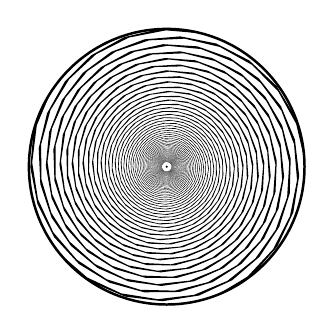
\begin{tikzpicture}
    % 多条紧密对数螺线黑带（致密同心环视觉幻觉，m = 0.048）
    \def\Rlim{1.75}
    \def\mval{0.048}
    \def\rstart{0.06}
    \def\dphi{18}
    \begin{scope}
      \clip (0,0) circle (\Rlim);
      \foreach \k in {0, 72, 144, 216, 288} {
        \fill[black]
          plot[domain=0:72, samples=260]
            ({\rstart*exp(\mval*\x)*cos(-\x r + \k)}, {\rstart*exp(\mval*\x)*sin(-\x r + \k)})
          --
          plot[domain=72:0, samples=260]
            ({\rstart*exp(\mval*\x)*cos(-\x r + \k + \dphi)}, {\rstart*exp(\mval*\x)*sin(-\x r + \k + \dphi)})
          -- cycle;
      }
    \end{scope}
    \draw[line width=0.9pt] (0,0) circle (\Rlim);
    \fill[white] (0,0) circle (0.045);
    \fill[black] (0,0) circle (0.015);
  \end{tikzpicture}
  \caption*{图\ 93.1}
\end{figure}

为什么会产生这样的幻觉呢？

\par\medskip\noindent
\begin{minipage}[c]{0.49\textwidth}
  \hspace{2em}我们来看图 93.2。图中画了两条对数螺线 $C_1$ 和 $C_2$，虚线画的 $C_2$ 是由实线画的 $C_1$ 绕极点 $O$ 旋转角 $\alpha$ 以后得到的。设 $B(\rho, \theta)$ 是 $C_1$ 上的任意点，
  \[
    \rho = e^{m\theta}.
  \]
\end{minipage}%
\hfill
\begin{minipage}[c]{0.47\textwidth}
  \centering
  \begin{tikzpicture}[scale=0.92]
    % C1: rho = R0 * exp(m*theta), m = 0.21, R0 = 1.35
    % C2 为 C1 绕 O 顺时针旋转 alpha = 45 度所得
    \def\mval{0.21}
    \def\Rzero{1.35}
    \def\alphadeg{45}
    % 实线 C1
    \draw[line width=0.85pt, curveblue, domain=-10.5:0.18, samples=220, smooth]
      plot ({\Rzero*exp(\mval*\x)*cos(\x r)}, {\Rzero*exp(\mval*\x)*sin(\x r)});
    % 虚线 C2（顺时针旋转 alpha）
    \begin{scope}[rotate=-\alphadeg]
      \draw[dashed, dash pattern=on 3pt off 2pt, line width=0.8pt, black, domain=-10.5:0.18, samples=220, smooth]
        plot ({\Rzero*exp(\mval*\x)*cos(\x r)}, {\Rzero*exp(\mval*\x)*sin(\x r)});
    \end{scope}

    % 极轴 OA、射线 OP（过 B 点）与射线 OP'（过 D, B' 点）
    \draw[line width=0.55pt] (0,0) -- (1.42,0);
    \draw[line width=0.6pt, -{Stealth[length=4pt]}] (0,0) -- (-22:1.85);
    \draw[line width=0.6pt, -{Stealth[length=4pt]}] (0,0) -- (-67:1.85);

    % 关键点坐标（弧度计算）
    \coordinate (A) at ({\Rzero}, 0);
    \pgfmathsetmacro{\rB}{\Rzero*exp(\mval*(-0.38397))}
    \coordinate (B) at (-22:\rB);
    \pgfmathsetmacro{\rC}{\Rzero*exp(\mval*(-0.78540))}
    \coordinate (C) at (-45:\rC);
    \pgfmathsetmacro{\rD}{\Rzero*exp(\mval*(-1.16937))}
    \coordinate (D) at (-67:\rD);
    \coordinate (Ap) at (-45:\Rzero);
    \coordinate (Bp) at (-67:\rB);

    \fill (0,0) circle (1.1pt) node[above right=0pt, fill=white, inner sep=0.4pt] {\footnotesize $O$};
    \fill (A) circle (1.2pt) node[above=1pt] {\footnotesize $A$};
    \fill (B) circle (1.2pt) node[below right=0pt, xshift=-1pt] {\footnotesize $B$};
    \fill (C) circle (1.2pt) node[below left=-2pt] {\footnotesize $C$};
    \fill (D) circle (1.2pt) node[above left=-1pt] {\footnotesize $D$};
    \fill (Ap) circle (1.2pt) node[below right=-1pt] {\footnotesize $A'$};
    \fill (Bp) circle (1.2pt) node[below left=-1pt] {\footnotesize $B'$};

    \node[right=1pt] at (-22:1.82) {\footnotesize $P$};
    \node[right=1pt] at (-67:1.78) {\footnotesize $P'$};
    \node at (-135:0.58) {\footnotesize $C_1$};
    \node at (-172:1.05) {\footnotesize $C_2$};
  \end{tikzpicture}
  \par\vspace{3pt}{\footnotesize 图\ 93.2}
\end{minipage}
\par\medskip

将 $B$ 绕 $O$ 旋转角 $\alpha$ 后，得到点 $B'(\rho, \theta_1)$，其中 $\theta_1 = \theta - \alpha$。因而 $\theta = \theta_1 + \alpha$，由此推出
\[
  OB' = \rho = e^{m(\theta_1 + \alpha)} = e^{m\theta_1 + m\alpha}.
\]
设 $D$ 是 $C_1$ 上极角为 $\theta_1$ 的点，其极半径为 $\rho_1$，则
\[
  OD = \rho_1 = e^{m\theta_1}.
\]
由此推出
\[
  \frac{OB'}{OD} = \frac{e^{m\theta_1 + m\alpha}}{e^{m\theta_1}} = e^{m\alpha} = \text{定值},
\]
这说明 $C_2$ 是 $C_1$ 的位似形，并且由于 $\alpha > 0$，$e^{m\alpha} > 1$，因而 $OB' > OD$，从 $D$ 到 $B'$ 的变换是放大\footnote{重排校订：原书此处误印作“从 $D$ 到 $B$”，据 $OB' > OD$ 及位似对应关系订正为 $B'$。}。

现在问题就很清楚了：可以用两种不同的变换把对数螺线 $C_1$ 变到 $C_2$，一种是旋转，它使 $C_1$ 的点 $B$ 对应于 $C_2$ 的点 $B'$；另一种是位似，它使 $C_1$ 的点 $D$ 对应于 $C_2$ 的点 $B'$。$B$ 与 $B'$ 相距较远，而 $D$ 与 $B'$ 则比较靠近。当我们目不转睛地注视着对数螺线 $C_1$ 的弧 $CD$ 时，随着曲线 $C_1$ 绕 $O$ 点转动到 $C_2$ 的位置，我们的视线仍停留在 $CD$ 附近，因而不易注意到 $C_2$ 的弧 $A'B'$ 是由 $C_1$ 的弧 $AB$ 旋转得来，相反却会误认为弧 $A'B'$ 是由弧 $CD$ 经过位似变换得来的。向一个方向旋转时，对应的位似变换是放大；向相反方向旋转时，对应的位似变换是缩小。

在布置科技画廊或商品橱窗时，可以利用对数螺线的上述性质逼真地表现光芒四射的形象。为此，需要在屏板上沿着极半径的方向每隔一定角度刻一条狭槽，这块屏板是固定不动的；在屏板后面放一块旋转的透明圆板，圆板上用深色画了若干条对数螺线；旋转透明板后面再放一只彩色灯泡，如图 93.3 所示。灯泡发出的光，穿过透明板，再从屏板的放射形狭槽里透出来，每一道狭槽都象是一道光芒。透明板上曲线的阴影，把每道狭槽所表现的光芒都隔断成几节。当透明板转动时，阴影从狭槽靠近中心的一端连续向另一端移动，看上去就好像一节一节的光芒源源不断地从屏板中心发出，射向四面八方，令人赞叹不已。

\begin{figure}[htbp]
  \centering
  \vspace*{3pt}
  \begin{tikzpicture}[scale=0.92]
    % 1. 左侧：固定透视屏板（刻有放射形狭槽）
    \begin{scope}[shift={(-2.3,0)}]
      % 屏板正面与厚度侧边
      \draw[line width=0.75pt] (-1.0,-0.85) -- (0.85,-0.55) -- (0.85,0.95) -- (-1.0,0.85) -- cycle;
      \draw[line width=0.55pt] (0.85,-0.55) -- (0.95,-0.52) -- (0.95,0.92) -- (0.85,0.95);
      \draw[line width=0.55pt] (-1.0,0.85) -- (-0.90,0.88) -- (0.95,0.92);
      % 中心及放射狭槽（透视压缩）
      \coordinate (C1) at (-0.08,0.10);
      \foreach \ang in {0,30,...,330} {
        \draw[line width=0.65pt, fill=white]
          ($(C1)+(\ang-4:0.22)$) -- ($(C1)+(\ang-5:0.65)$)
          -- ($(C1)+(\ang+5:0.65)$) -- ($(C1)+(\ang+4:0.22)$) -- cycle;
      }
      % 中心星形孔
      \draw[line width=0.6pt, fill=white]
        ($(C1)+(0:0.18)$) -- ($(C1)+(36:0.08)$) -- ($(C1)+(72:0.18)$)
        -- ($(C1)+(108:0.08)$) -- ($(C1)+(144:0.18)$) -- ($(C1)+(180:0.08)$)
        -- ($(C1)+(216:0.18)$) -- ($(C1)+(252:0.08)$) -- ($(C1)+(288:0.18)$)
        -- ($(C1)+(324:0.08)$) -- cycle;
    \end{scope}

    % 2. 中间：旋转透明圆板（画有若干条深色对数螺线）
    \begin{scope}[shift={(0.25,0.12)}]
      \begin{scope}[xscale=0.88]
        \clip (0,0) circle (0.95);
        \foreach \k in {0,60,120,180,240,300} {
          \fill[black!85]
            plot[domain=-2.5:3.8, samples=70]
              ({0.14*exp(0.55*\x)*cos(\x r + \k)}, {0.14*exp(0.55*\x)*sin(\x r + \k)})
            --
            plot[domain=3.8:-2.5, samples=70]
              ({0.14*exp(0.55*\x)*cos(\x r + \k + 25)}, {0.14*exp(0.55*\x)*sin(\x r + \k + 25)})
            -- cycle;
        }
      \end{scope}
      \draw[line width=0.75pt] (0,0) ellipse (0.836 and 0.95);
      \fill[white, draw=black, line width=0.55pt] (0,0) circle (0.09);
      \fill (0,0) circle (0.03);
      % 底部旋转箭头
      \draw[line width=0.6pt, -{Stealth[length=3.5pt]}] (-0.42,-1.10) arc (-125:-55:0.75);
    \end{scope}

    % 3. 右侧：彩色灯泡及光芒虚线
    \begin{scope}[shift={(2.15,0.15)}]
      % 灯泡玻璃泡
      \draw[line width=0.7pt, fill=white]
        (-0.14,-0.32) .. controls (-0.18,-0.10) and (-0.36,0.05) .. (-0.36,0.32)
        arc (180:0:0.36)
        .. controls (0.36,0.05) and (0.18,-0.10) .. (0.14,-0.32) -- cycle;
      % 灯头螺旋底座
      \draw[line width=0.7pt] (-0.14,-0.32) -- (-0.14,-0.52) -- (0.14,-0.52) -- (0.14,-0.32);
      \draw[line width=0.5pt] (-0.14,-0.39) -- (0.14,-0.39);
      \draw[line width=0.5pt] (-0.14,-0.46) -- (0.14,-0.46);
      \draw[line width=0.6pt] (-0.08,-0.52) -- (0,-0.59) -- (0.08,-0.52);
      % 内部灯丝
      \draw[line width=0.45pt] (-0.07,-0.25) -- (-0.09,0.22)
        .. controls (-0.04,0.32) and (0.04,0.32) .. (0.09,0.22) -- (0.07,-0.25);
      % 放射光芒短线
      \foreach \ang in {-35,-10,15,40,65,90,115,140,165,190,215} {
        \draw[line width=0.55pt] (\ang:0.50) -- (\ang:0.72);
      }
    \end{scope}
  \end{tikzpicture}
  \caption*{图\ 93.3}
\end{figure}

幻灯和电影也都可以利用类似的方法产生光芒四射的效果。
